% Written by Peter Goetz, August 2020 for Math 102
\documentclass[12pt]{amsart}
\usepackage{amssymb, latexsym,xspace}
\usepackage[pdftex]{graphicx}
\usepackage{amsmath}
\usepackage{soul} % for highlights-- command is \hl
\usepackage{xcolor}

%%%%%%%%%%%%%%%%%%%%%%%
%
% Change course, date, etc. here and the 
% header will be automatically generated.
%
%%%%%%%%%%%%%%%%%%%%%%%
\newcommand{\class}{Math 102}
\newcommand{\term}{Precalculus}
\newcommand{\quiztitle}{Problem Set 2: Graphs of Functions, Average Rate of Change, Algebra with Functions}
%%%%%%%%%%%%%%%%%%%%


%%%%%% Small margin to leave room for students' work %%%%%%%
\usepackage[margin=0.75in,top=0.5in,
            nohead,
            pdftex]{geometry}

%%%%%% Various PDF commands; generally not needed in a quiz %%%%%%%
\usepackage[pdftex, colorlinks=true,
            linkcolor=blue, citecolor=blue,
            urlcolor=blue, letterpaper,
            pdftitle={},
            pdfpagemode=None]{hyperref}

%%%%% spread the lines out a bit.
\pagestyle{plain}
\linespread{1.3}
\parindent 0ex

\begin{document}
%%%%%%%%% Header %%%%%%%%%%%
\textbf{\class \xspace\xspace \term \xspace\xspace - \quiztitle\\}
%\quizdate\xspace\xspace - \timelimit \hspace{1.5in} Name: }\\
\rule[1ex]{\textwidth}{.1pt}


%These problems cover material in Sections 2.4, 2.5, 2.6 on graphs of functions, average rate of change, and algebra with functions.

%{\bf Due date}: September 11, 2020

\begin{enumerate}

\item Let $f(x) = \frac{1}{3} x + 2$.
\begin{itemize}
\item[(a)] Fill in the following table.
\begin{tabular}{| c | c | c | c | c | c |}
\hline
$x$ & $-6$ & $-3$ & $0$ & $3$ & $6$ \\
\hline
$f(x)$ & \ \   & \ \  & \ \  & \ \  & \ \ \\
\hline
\end{tabular}
\item[(b)] Use your table to graph this function.
\item[(c)] Determine the domain of $f(x)$.
\item[(d)] Determine the range of $f(x)$. 
\end{itemize}

\item Let $f(x) = \sqrt{ 2 x}$.

\begin{itemize}
\item[(a)] Fill in the following table.
\begin{tabular}{| c | c | c | c | c | c |}
\hline
$x$ & $0$ & $2$ & $\frac{9}{2}$ & $8$ & $18$ \\
\hline
$f(x)$ & \ \   & \ \  & \ \  & \ \  & \ \ \\
\hline
\end{tabular}
\item[(b)] Use your table to graph this function.
\item[(c)] Determine the domain of $f(x)$.
\item[(d)] Determine the range of $f(x)$. 
\end{itemize}

\item Let $g(x) = x^2-2$.
\begin{itemize}
\item[(a)] Graph this function.
\item[(b)] What is its domain?
\item[(c)] What is its range? Write your answer in interval notation.
\end{itemize}

\item Let $$f(x) = \begin{cases}  x+4 \quad & x \leq 2 \\ 4 & x > 2. \end{cases}$$ 
\begin{itemize}
\item[(a)] Graph this function. Hint: Start by making a table of some values of this function.
\item[(b)] What is its domain?
\item[(c)] What is its range? Write your answer in interval notation.
\end{itemize}

\item Let $$f(x) = \begin{cases}  x^2 \qquad & -1 \leq x \leq 2 \\ -2 & 2< x\leq 3 \\ x+1 & x > 3. \end{cases}$$ 
\begin{itemize}
\item[(a)] Graph this function. Hint: Start by making a table of some values of this function.
\item[(b)] What is its domain? Write your answer in interval notation.
\item[(c)] What is its range? Write your answer in interval notation.
\end{itemize}
\eject

\item Use the graph of $y = f(x)$ below to answer the following questions.

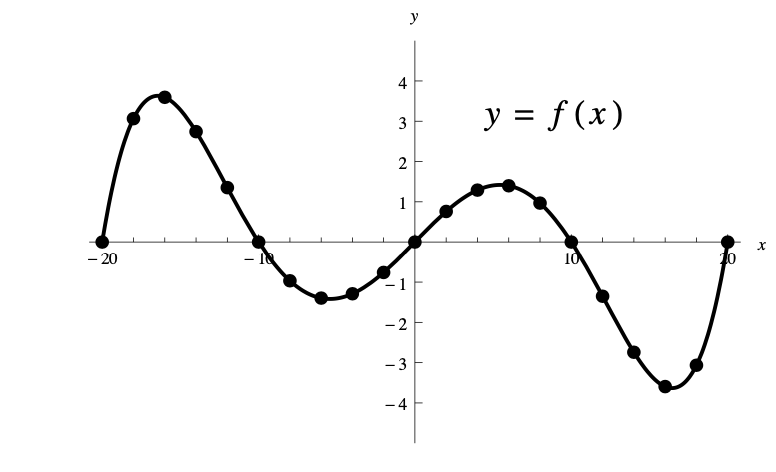
\includegraphics[scale=.7]{graph_for_problem_3.png}

\begin{itemize}
\item[(a)] Evaluate $f(-18)$.
\item[(b)] Is $f(6) < 0$? Explain briefly.
\item[(c)] Determine all of the zeros.
\item[(d)] Determine the $y$-intercept. 
\item[(e)] How many solutions does the equation $f(x) = 1$ have?
\end{itemize}

\item Let $f(x) = 2 | x | +1$.

\begin{itemize}
\item[(a)] Graph this function.
\item[(b)] Explain why your graph shows that $f(x)$ is an even function.
\item[(c)] Show, algebraically, that $f(x)$ is an even function.
\end{itemize}

\item Let $g(x) = x^3-x$.

\begin{itemize}
\item[(a)] Graph this function.
\item[(b)] Explain why your graph shows that $g(x)$ is an odd function.
\item[(c)] Show, algebraically, that $g(x)$ is an odd function.
\end{itemize}

\item Let $h(x) = |x-3| - 2$.
\begin{itemize}
\item[(a)] Use the graph of $h(x)$ to determine if $h(x)$ is an even function, an odd function, or neither.
\item[(b)] Use algebra to determine if $h(x)$ is an even function, an odd function, or neither.
\item[(c)] Which method, (a) or (b), do you prefer? Explain briefly. 
\end{itemize}

\item Suppose that $f(x)$ is an odd function and $0$ is in the domain of $f(x)$. What is $f(0)$ equal to? Explain your reasoning either using a graph or by using algebra. 
\eject

\item Use the graph of $y = f(x)$ below to answer the following questions.

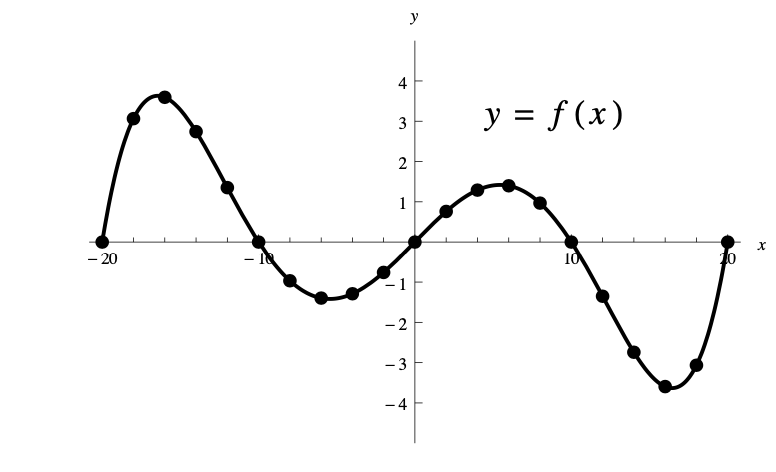
\includegraphics[scale=.7]{graph_for_problem_3.png}

\begin{itemize}
\item[(a)] Is $f(x)$ an even function? Explain briefly. 
\item[(b)] Determine the interval(s) on which $f(x)$ is increasing.
\item[(c)] Determine the interval(s) on which $f(x)$ is decreasing.
\item[(d)] Are there any intervals where $f(x)$ is constant?
\end{itemize}

\item Let $g(x) = -2x^2+ x + 5$. Determine the average rate of change of $g(x)$ on the interval $[-2, 3]$. 

\item Use the following table to determine the average rate of change of $h(x)$ on the interval $[2, 6]$.
\begin{tabular}{| c | c | c | c | c | c |}
\hline
$x$ & $0$ & $1$ & $2$ & $5$ & $6$ \\
\hline
$h(x)$ & -3  & -1  & 2.4  & 7  & 10.5 \\
\hline
\end{tabular}

\item Suppose that the function $f(x)$ is constant on the interval $[a, b]$. What is the average rate of change of $f(x)$ on this interval? Explain your reasoning.

\item Let $f(x) = 3x^2- 2$. Let $g(x) = \frac{1}{x+1}$.

\begin{itemize}
\item[(a)] Determine $f(x) + g(x)$. What is the domain?
\item[(b)] Determine $f(x) - g(x)$. What is the domain?
\item[(c)] Determine $f(x)g(x)$. What is the domain?
\item[(d)] Determine $\frac{f(x)}{g(x)}$. What is the domain? (Be careful.)
\end{itemize}

\item Let $f(x) = x^2+x$, let $g(x) = \sqrt{x}$. 

\begin{itemize}
\item[(a)] Determine $(f \circ g)(x)$.
\item[(b)] Evaluate $(f \circ g)(1)$ and $(f \circ g)(\frac{9}{4})$.
\item[(c)] Determine $(g \circ f)(x)$.
\item[(d)] Evaluate $(g \circ f)(2)$ and $(g \circ f)(-3)$.
\end{itemize}

\item Use the tables below to answer the following questions. Some of the answers might be undefined, if so write ``undefined".

\begin{tabular}{| c | c | c | c | c | c |}
\hline
$x$ & $5$ & $6$ & $7$ & $8$ & $9$ \\
\hline
$f(x)$ & 8   & 7  & 6  & 5  & 4 \\
\hline
\end{tabular} \hspace{3cm}
\begin{tabular}{| c | c | c | c | c | c |}
\hline
$x$ & $5$ & $6$ & $7$ & $8$ & $9$ \\
\hline
$g(x)$ & 7   & 8  & 6  & 5  & 4 \\
\hline
\end{tabular}

\begin{itemize}
\item[(a)] Evaluate $(f \circ g)(6)$.
\item[(b)] Evaluate $(g \circ f)(8)$.
\item[(c)] Evaluate $(f \circ f)(5)$.
\item[(d)] Evaluate $(g \circ g)(6)$.
\item[(e)] Evaluate $(f \circ g)(9)$.
\item[(f)] Determine all solutions to the equation $f(x+2) = 4$
\end{itemize}

\item Let $h(x) = \sqrt[3]{4x^2-1}$. Find two functions $f(x)$ and $g(x)$ such that $h(x) = (f \circ g)(x)$.

\item The volume of a spherical balloon of radius $r$ cm is given by $$V(r) = (4/3) \pi r^3 \text{ cm}^3.$$ Suppose that the balloon is inflated so that its radius increases from $r = 1$ cm at time $t = 0$ seconds at a constant rate of $2$ cm per second.

\begin{itemize}
\item[(a)] Find a function $r(t)$ that gives the radius of the balloon (in cm) as a function of time (in seconds). Hint: This should be a linear function.
\item[(b)] Determine a function $V(t)$ that gives the volume of the balloon in (cm$^3$) as a function of time (in seconds).
\item[(c)] Determine the volume of the balloon after $2$ seconds. 
\end{itemize}

\item Klamath Connections students at HSU recently finished an experiment to determine the effects of nitrogen and phosphorus on algae growth.  They added nitrogen and phosphorus (common ingredients in fertilizer) to Klamath river water and recorded an opacity score (how cloudy) for the water every 3 days. We expect the negative control to have a low opacity score which means it is more transparent than water with added nitrogen and phosphorus.  Summarizing: negative control is Klamath water without nitrogen and phosphorus added, treatment is Klamath water with nitrogen and phosphorus added, positive control is a commercial growth medium with nutrients and pH optimized for algal growth. 

The results look something like this:

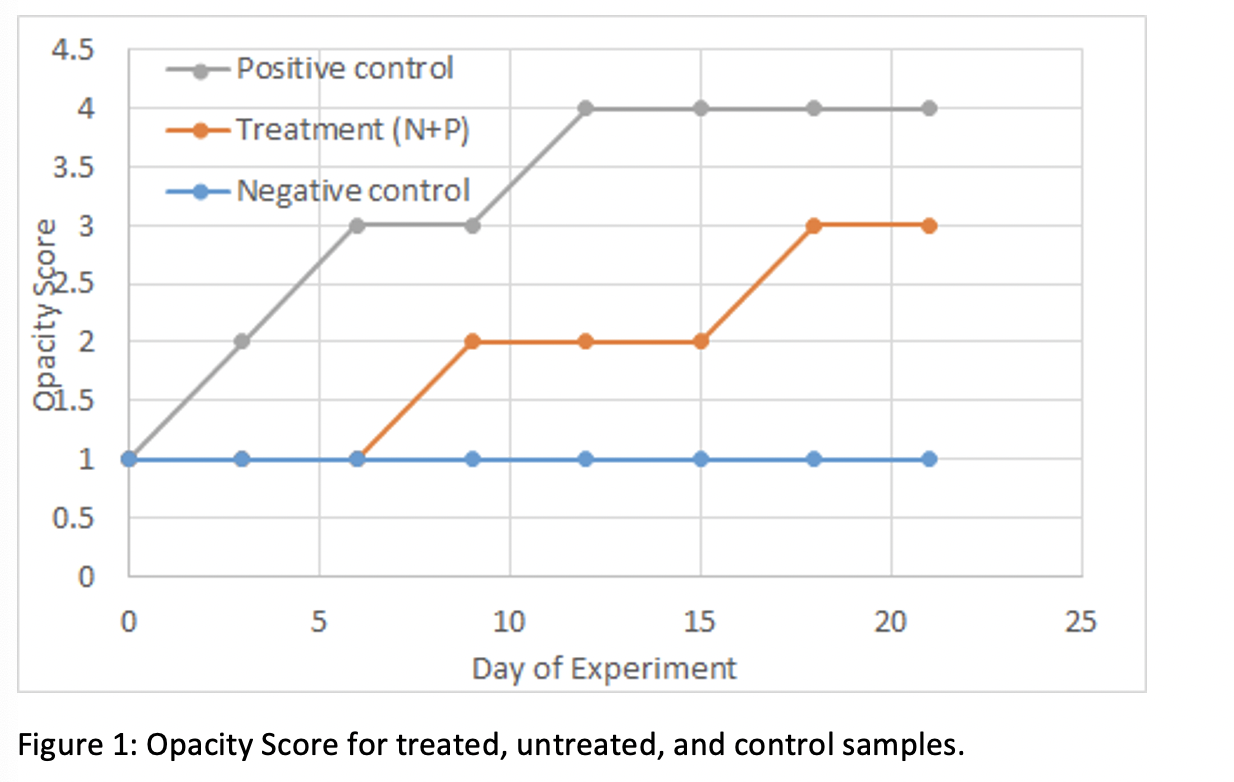
\includegraphics[scale=0.5]{KC_opacity_graph}

Using this graph answer the following questions. Note that you can {\bf ignore} the graph for the {\bf positive control}. 

\begin{itemize}
\item[(a)] What is the average rate of change for treated samples over the 21 days?
\item[(b)] What is the average rate of change for untreated samples (negative control) over the 21 days?
\item[(c)] Determine a piece-wise function that models the treated samples. Use correct function notation. For example, for a start:
$$O(t) = \begin{cases} \ \ \ \  & t<6, \\ \ \ \ \   &6 \leq t < 9, \\ \ \ \ \   & \ \ \ \ \ \ \ \ \ \ \ \  , \\ \ \ \  &  \ \ \ \ \ \ \ \ \ \ \ \ . \end{cases}$$
\item[(d)] Why is a piece-wise function a good way to model the treated samples?
\item[(e)] Determine a function, $N(t)$, that models the untreated samples (negative control). 
\item[(f)] Determine $O(21)$. 
\item[(g)] Determine $N(21)$.
\item[(h)] What do your answers to parts (f) and (g) tell you about the affect of adding nitrogen and phosphorus to river water?
\end{itemize}


\item The following puzzle appeared in Season 9, Episode 17 of the Simpsons.  
\begin{figure}[ht]
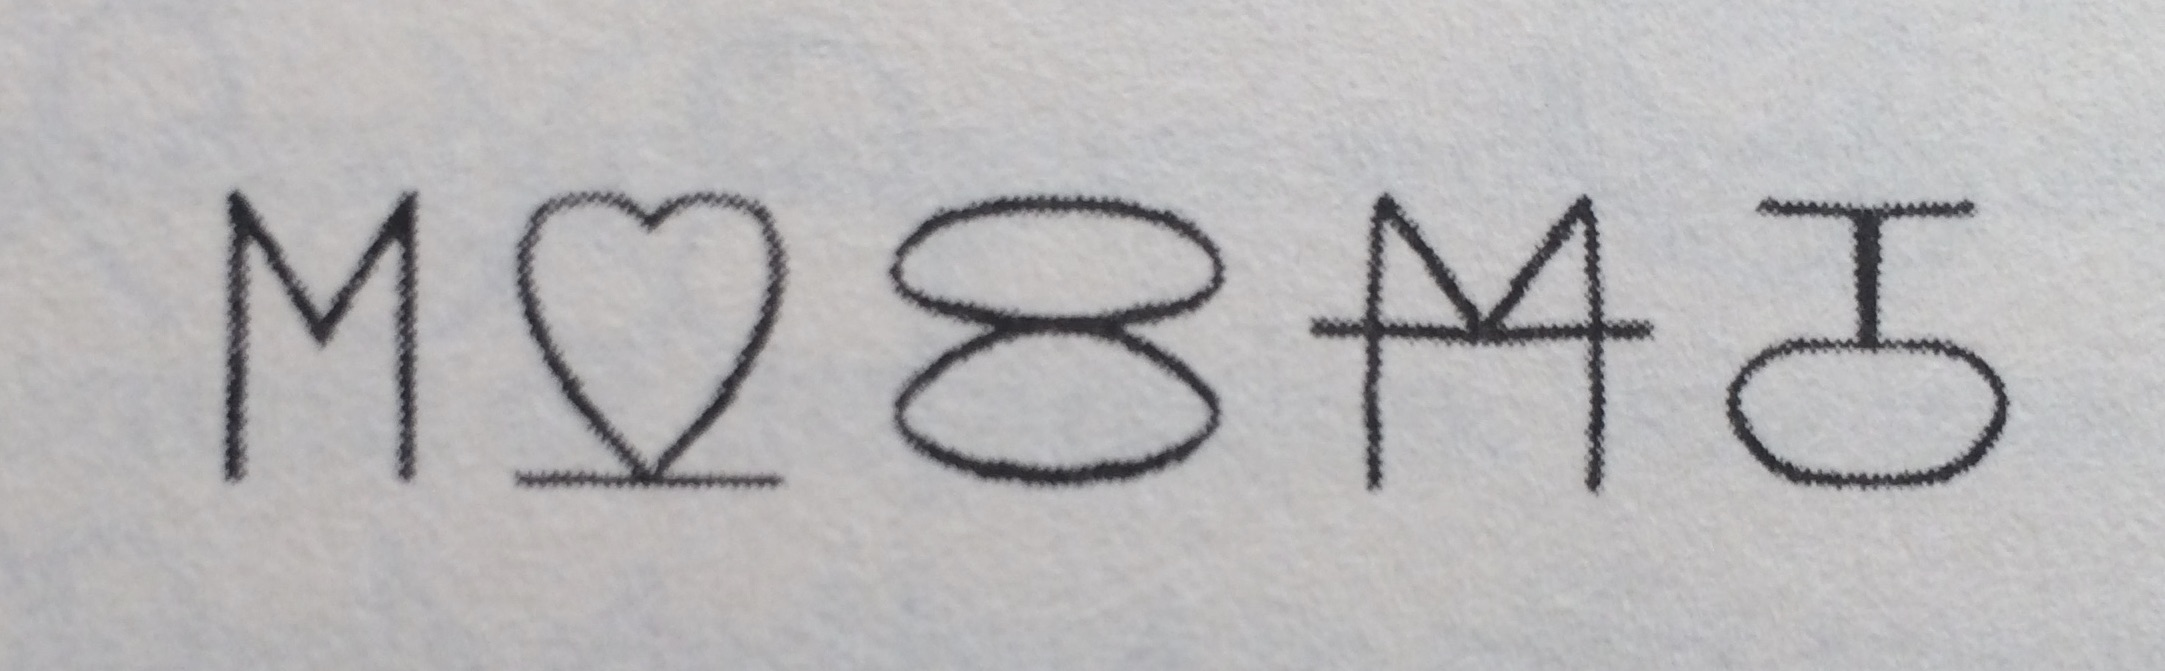
\includegraphics[scale=0.05]{simpsons}
\end{figure}

\begin{enumerate}
\item Can you find the next term in the sequence?  Hint: each term has symmetry.  If you cover the left half of each term, this might help you see the solution.
\item Which of the terms could be a graph of a function?  Hint: apply the vertical line test.
\end{enumerate}


\item REFLECTION AND CONSOLIDATION (Hint: this will form part of a study guide for your first exam!)
\begin{enumerate}
\item Summarize the main ideas/formulas you used for this problem set.  You can list formulas, bullet-out phrases, write a paragraph, draw sketches, or answer this question in any way that makes sense to you.
\item What three problems were the most challenging for you?  After deciding, look at your solutions carefully, and write a short explanation of what you found challenging and how you overcame this challenge in your problem solving.  For example, did you find a simpler problem about the same topic?  Did you guess and check?  Did you graph with technology?
\item Write three potential test questions on the topics covered in this problem set.
\end{enumerate}
      

\end{enumerate}


\end{document}